\newcommand{\figureArray}[1]{
  \def\lang{\detokenize{#1}}
  \def\langRu{\detokenize{ru}}
  \def\langEn{\detokenize{en}}
  \def\figureCaption{XXX: No translation.}
  \ifx \lang\langRu
  \def\figureCaption{
    Схематическое изображение массива 4x20 (4 строки, 20 столбцов.)
  }
  \fi
  \ifx \lang\langEn
  \def\figureCaption{
    A schematic representation of a 2-dimensional array 4x20 (4 rows, 20
    columns.)
  }
  \fi
  \begin{figure}[ht]
    \centering
    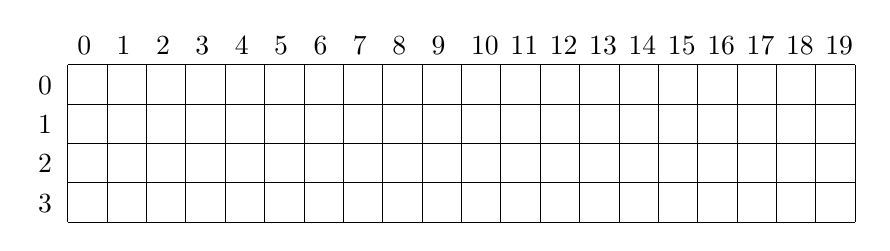
\begin{tikzpicture}
      \draw[step=0.5cm,black,very thin] (-5, -2) grid (5, 0);
      \foreach[count=\n from 0] \x in {-5, -4.5, ..., 4.5} {
        \draw (\x cm, 0) node[anchor=south west] {$\n$};
      }
      \foreach[count=\n from 0] \y in {-0.5, -1.0, ..., -2} {
        \draw (-5.5, \y) node[anchor=south west] {$\n$};
      }
    \end{tikzpicture}
    \caption{\figureCaption}
    \label{fig:2d-array-example}
  \end{figure}
}
